\documentclass[10pt]{beamer}


\usetheme[progressbar=frametitle]{metropolis}
\usepackage{appendixnumberbeamer}

\usepackage{animate}
\usepackage{beamerbaseoverlay}
\usepackage{booktabs}
\usepackage[scale=2]{ccicons}

\usepackage{pgfplots}
\usepgfplotslibrary{dateplot}

\usepackage{xspace}
\newcommand{\themename}{\textbf{\textsc{metropolis}}\xspace}

\title{Formalisation of constructable numbers}
\subtitle{Third lecture regarding the Bachelor thesis}
% \date{\today}
\date{}
\author{Ludwig Monnerjahn}
%\institute{Center for modern beamer themes}
% \titlegraphic{\hfill\includegraphics[height=1.5cm]{logo.pdf}}

% % Remove navigation bar
% \setbeamertemplate{navigation symbols}{}

% % Tikz package
% \usepackage{tikz}
% \usetikzlibrary{positioning}

\usepackage[T1]{fontenc}
\usepackage[utf8]{inputenc}
\usepackage{listings}
\usepackage{amssymb}
\usepackage{amsmath}
\usepackage{amsthm}
\usepackage{hyperref}
\usepackage{etexcmds}
\usepackage{thmtools}
\usepackage{tikz-cd}
\usepackage{wrapfig}
\usepackage{graphicx}

%tikz 
\definecolor{Acolor}{RGB}{104,129,174}
\definecolor{Bcolor}{RGB}{227,118,59}
\definecolor{Ccolor}{RGB}{169,183,209}
\definecolor{medgrey}{RGB}{150,150,150}


%lean highlight
\usepackage{color}
\definecolor{keywordcolor}{rgb}{0.7, 0.1, 0.1}   % red
\definecolor{tacticcolor}{rgb}{0.0, 0.1, 0.6}    % blue
\definecolor{commentcolor}{rgb}{0.4, 0.4, 0.4}   % grey
\definecolor{symbolcolor}{rgb}{0.0, 0.1, 0.6}    % blue
\definecolor{sortcolor}{rgb}{0.1, 0.5, 0.1}      % green
\definecolor{attributecolor}{rgb}{0.7, 0.1, 0.1} % red

\def\lstlanguagefiles{lstlean.tex}
% set default language
\lstset{language=lean}

% % theorem style
% \theoremstyle{definition}
% \newtheorem*{theorem*}{Theorem}
% \newtheorem{proposition}[theorem]{Proposition}
% \newtheorem{problem}[theorem]{Problem}

% Remove blueprint commands
\newcommand{\uses}[1]{}
\newcommand{\proves}[1]{}
\newcommand{\discussion}[1]{}
\newcommand{\lean}[1]{}
\newcommand{\leanok}{}
\newcommand{\mathlibok}{}
\newcommand{\notready}{}

%Notaion
\newcommand{\dist}{\text{ dist }}
\newcommand{\N}{\mathbb{N}}
\newcommand{\R}{\mathbb{R}}
\newcommand{\C}{\mathbb{C}}
\newcommand{\Q}{\mathbb{Q}}
\newcommand{\Z}{\mathbb{Z}}

\tikzset{
            carc/.style args={#1:#2:#3}{
              insert path={+(#1:#3) arc (#1:#2:#3)}
            }
          }

\begin{document}
\maketitle

\begin{frame}{Table of contents}
  \setbeamertemplate{section in toc}[sections numbered]
  \tableofcontents%[hideallsubsections]
\end{frame}

\section{Defintions}
\begin{frame}[fragile]
    %\color{white}\vrule width\paperwidth height\paperheight
    \begin{figure}[h]
        \centering
        \scalebox{0.3}{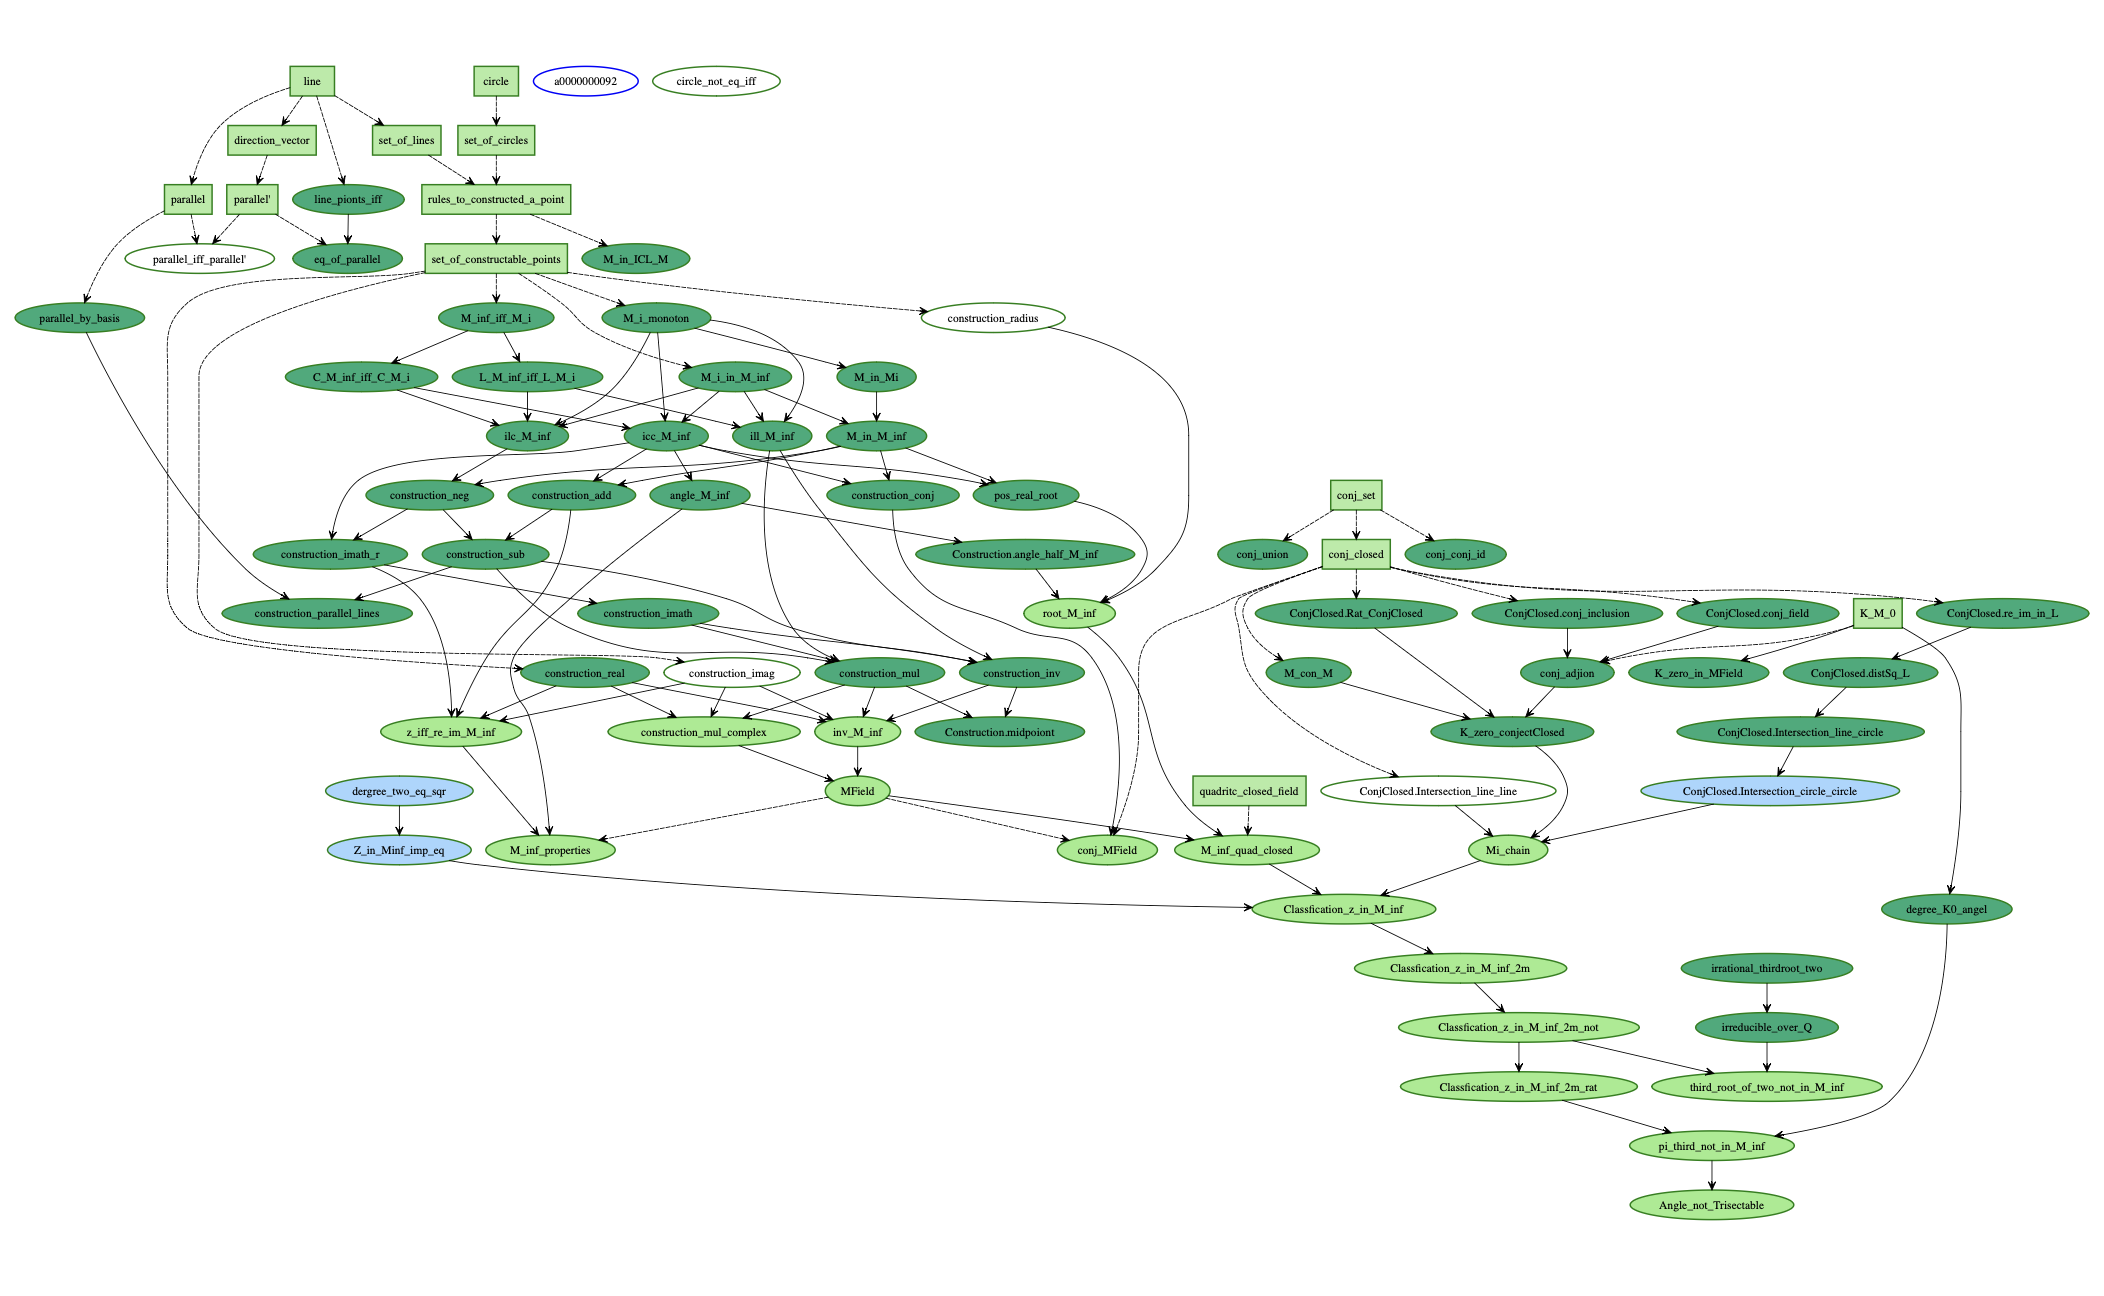
\includegraphics[angle=0]{slides/DependencyGraph}}
        \label{fig:DependencyGraph}
        \caption{Dependency Graph}
    \end{figure}
\end{frame}
\begin{frame}[fragile]
    \begin{definition}[Line]
        \label{def:line}
        A line $l$ through two points $x,y\in\mathbb{C}$ with $x\ne y$ is defined by the set: $$l:=\{\lambda x+(1-\lambda)y\mid\lambda\in\mathbb{R}\}.$$
    \end{definition}

    \begin{lstlisting}
        structure line where
            (z₁ z₂ : ℂ)
    
        def line.points (l: line) : Set ℂ:= 
            {(t : ℂ) * l.z₁ + (1-t) * l.z₂ | (t : ℝ)}
    \end{lstlisting}

\end{frame}

\begin{frame}[fragile]
    \begin{definition}[Circle]
        \label{def:circle}
        A circle $c$ with center $z\in\mathbb{C}$ and radius $r\in\mathbb{R}_{\ge 0}$ is defined by the set: $$c:=\{z\in\mathbb{C} \mid\|z-c\|=r\}.$$
    \end{definition}
    
    \begin{lstlisting}
        structure circle where
            (c : ℂ)
            (r : ℝ)
    
        def circle.points (c: circle) := Metric.sphere c.c c.r
        noncomputable def circle.points' (c: circle) := 
            (⟨c.c, c.r⟩ : EuclideanGeometry.Sphere ℂ)
    \end{lstlisting}
\end{frame}

\begin{frame}[fragile]    
    \begin{definition}[Set of lines and circles]
        \label{def:set_of_lines_and_circles}
        $\mathcal{L(M)}$ is the set of all real straight lines defined by two points in $\mathcal{M}$.\\
        And $\mathcal{C(M)}$ is the set of all circles defined by a center in $\mathcal{M}$ and a radius equal to the distance between two points in $\mathcal{M}$.
    \end{definition}

    \begin{lstlisting}
    def L (M:Set ℂ): Set line := 
        {l |∃ z₁ z₂, l = {z₁ := z₁, z₂ := z₂} ∧ z₁ ∈  M ∧ z₂ ∈ M ∧ z₁ ≠ z₂}
    def C (M:Set ℂ): Set circle := 
        {c |∃ z r₁ r₂, c = {c:=z, r:=(dist r₁ r₂)} ∧ z ∈ M ∧ 
        r₁ ∈ M ∧ r₂ ∈ M}
    \end{lstlisting}
\end{frame}


\begin{frame}[fragile]
    \begin{definition}[Rules to construct a point]
        \label{def:rules_to_constructed_a_point}
        We define operations that can be used to construct new points.
        \begin{enumerate}
            \item $(ILL)$ is the intersection of two different lines in $\mathcal{L(M)}$.
            \item $(ILC)$ is the intersection of a line in $\mathcal{L(M)}$ and a circle in $\mathcal{C(M)}$.
            \item $(ICC)$ is the intersection of two different circles in $\mathcal{C(M)}$.
        \end{enumerate}
        $ICL(\mathcal{M})$ is the set $\mathcal{M}$ combined with all points that can be constructed using the operations $(ILL)$, $(ILC)$ and $(ICC)$.
    \end{definition}
    
    \begin{lstlisting}
    def ill (M:Set ℂ): Set ℂ := 
        { z  |∃l₁ ∈ L M, ∃ l₂ ∈ L M,  z ∈ l₁.points ∩ l₂.points ∧ 
        l₁.points ≠ l₂.points}
    def ilc (M:Set ℂ): Set ℂ := 
        { z  |∃c ∈ C M, ∃ l ∈ L M,  z ∈ c.points ∩ l.points}
    def icc (M:Set ℂ): Set ℂ := 
        { z  |∃c₁ ∈ C M, ∃ c₂ ∈ C M,  z ∈ c₁.points ∩ c₂.points ∧ 
        c₁.points' ≠ c₂.points'}    
    
    def ICL_M (M : Set ℂ) : Set ℂ := M ∪ ill M ∪ ilc M ∪ icc M
    \end{lstlisting}
\end{frame}


\begin{frame}[fragile]
    \begin{definition}[Set of constructible points]
        \label{def:set_of_constructable_points}
        We define inductively the chain
        \begin{equation*}
            \mathcal{M}_0 \subseteq \mathcal{M}_1 \subseteq \mathcal{M}_2 \subseteq \dots
        \end{equation*}
        with $\mathcal{M}_0 = \mathcal{M}$ and $\mathcal{M}_{n+1} = ICL(\mathcal{M}_n)$.\newline
        And call $\mathcal{M}_{\infty} = \bigcup_{n \in \mathbb{N}} \mathcal{M}_n$ the set of all constructable points.
    \end{definition}
    
    \begin{lstlisting}
        def M_I (M : Set ℂ) : ℕ → Set ℂ
            | 0 => M
            | (Nat.succ n) => ICL_M (M_I M n)
    
        def M_inf (M : Set ℂ) : Set ℂ :=  ⋃ (n : ℕ), M_I M n
    \end{lstlisting}    
\end{frame}
\section{Field of constructable numbers}
\begin{frame}[fragile]
    %\color{white}\vrule width\paperwidth height\paperheight
    \begin{figure}[h]
        \centering
        \scalebox{0.3}{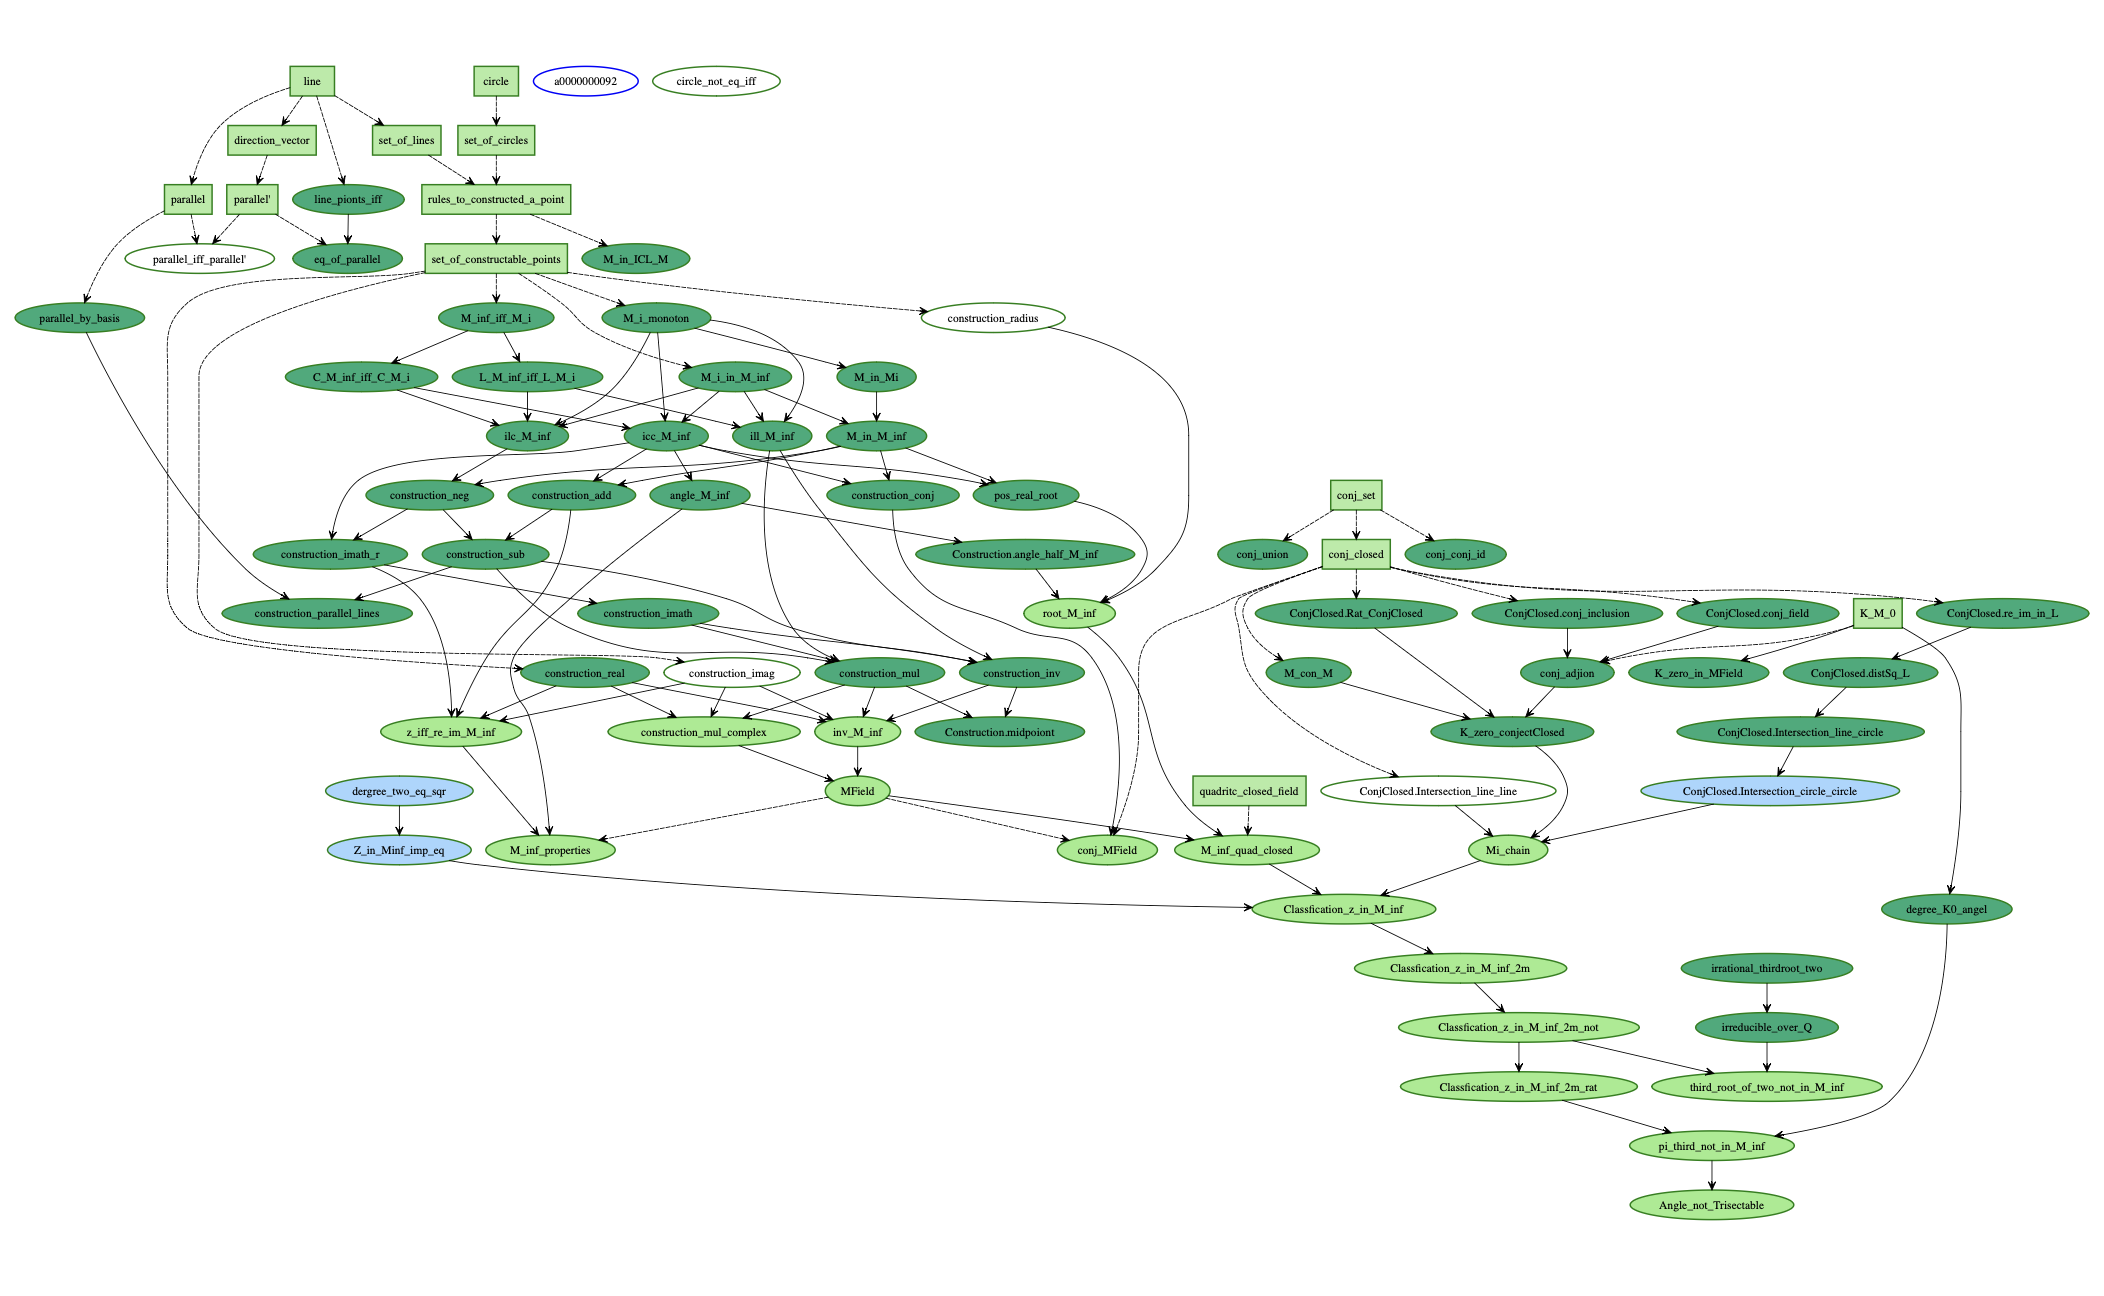
\includegraphics[angle=0]{slides/DependencyGraph}}
        \label{fig:DependencyGraph}
        \caption{Dependency Graph}
    \end{figure}
\end{frame}
\begin{frame}[fragile]
    \begin{definition}[quadratic closed field]
        \label{def:quadritc_closed_field}
        \leanok
        \lean{QuadraticClosed}
        A field $F$ is called \emph{quadratic closed} if for all $x \in F$ there is a $y \in F$ such that $y^2 = x$.
    \end{definition}

    \begin{lemma}
        \label{lem:M_inf_quad_closed}
        \leanok
        \lean{MField_QuadraticClosed, MField_QuadraticClosed_def}
        \uses{def:set_of_constructable_points, def:quadritc_closed_field}
        For $M\subseteq \mathbb{C}$ with $0,1 \in M$, $M_{\infty}$ is quadratic closed.
    \end{lemma}
    \scalebox{0.8}{\begin{minipage}{1.20\textwidth}

    \begin{figure}
    \centering
    \begin{tikzpicture}
        \draw[->] (-1,0) -- (7,0) node[right] {$\Re$};
        \draw[->] (0,-1) -- (0,4) node[above] {$\Im$};
        \coordinate[label=-135:$0$] (zero) at (0,0);
        \coordinate[label=-90:$1$] (one) at (1,0);
        \coordinate[label=-45:$r$] (r) at (6,0);
        \coordinate[label=-90:$\frac{r}{2}$] (r2) at (3,0);
        \coordinate[label=135:] (sqrt1) at (1,2.2360679775);
        \coordinate[label=135:$\sqrt{r}$] (sqrt) at (2.4494897428,0);
        \fill[black] (zero) circle (1pt);
        \fill[black] (one) circle (2pt);
        \fill[black] (r) circle (2pt);
        \fill[black] (r2) circle (2pt);
        \fill[black] (sqrt1) circle (2pt);
        \draw (r2) [carc=-10:190:3];
        \draw (zero) [carc=-10:80:2.4494897428];
        \draw (one) -- (sqrt1);
        \fill[red] (sqrt) circle (3pt);
    \end{tikzpicture}
    \caption{Construction of $\sqrt{r}$}
    \label{Fig.root}
    \end{figure}

    \end{minipage}}
\end{frame}

\begin{frame}
    \begin{definition}
        \label{def:conj_set}
        \leanok
        \lean{conj_set}
        For a Set $M \subset \mathbb{C}$ we define the \emph{conjugate set} of $M$ as 
        \begin{equation*}
            Conj(M) = \{\overline{z}\mid z\in M\}
        \end{equation*}
    \end{definition}
    
    \begin{definition}
        \label{def:conj_closed}
        \leanok
        \lean{ConjClosed}
        \uses{def:conj_set}
        We call a subset of $\C$ \emph{conjugate closed} if $M= Conj(M)$.
    \end{definition}
\end{frame}

\begin{frame}
    \begin{theorem}
        Let $K$ be an conjugation closed intermediate field of $\mathbb{Q}$ and $\mathbb{C}$.
        \begin{itemize}
            \item If $z\in ill(K)$ then $z\in K$.
            \item If $z\in ilc(K)$ then there exist $w^2 \in K$ such that $z\in K(w)$.
            \item If $z\in icc(K)$ then there exist $w^2 \in K$ such that $z\in K(w)$.
        \end{itemize}
    \end{theorem}
\end{frame}


\begin{frame}[fragile]
    %\color{white}\vrule width\paperwidth height\paperheight
    \begin{figure}[h]
        \centering
        \scalebox{0.3}{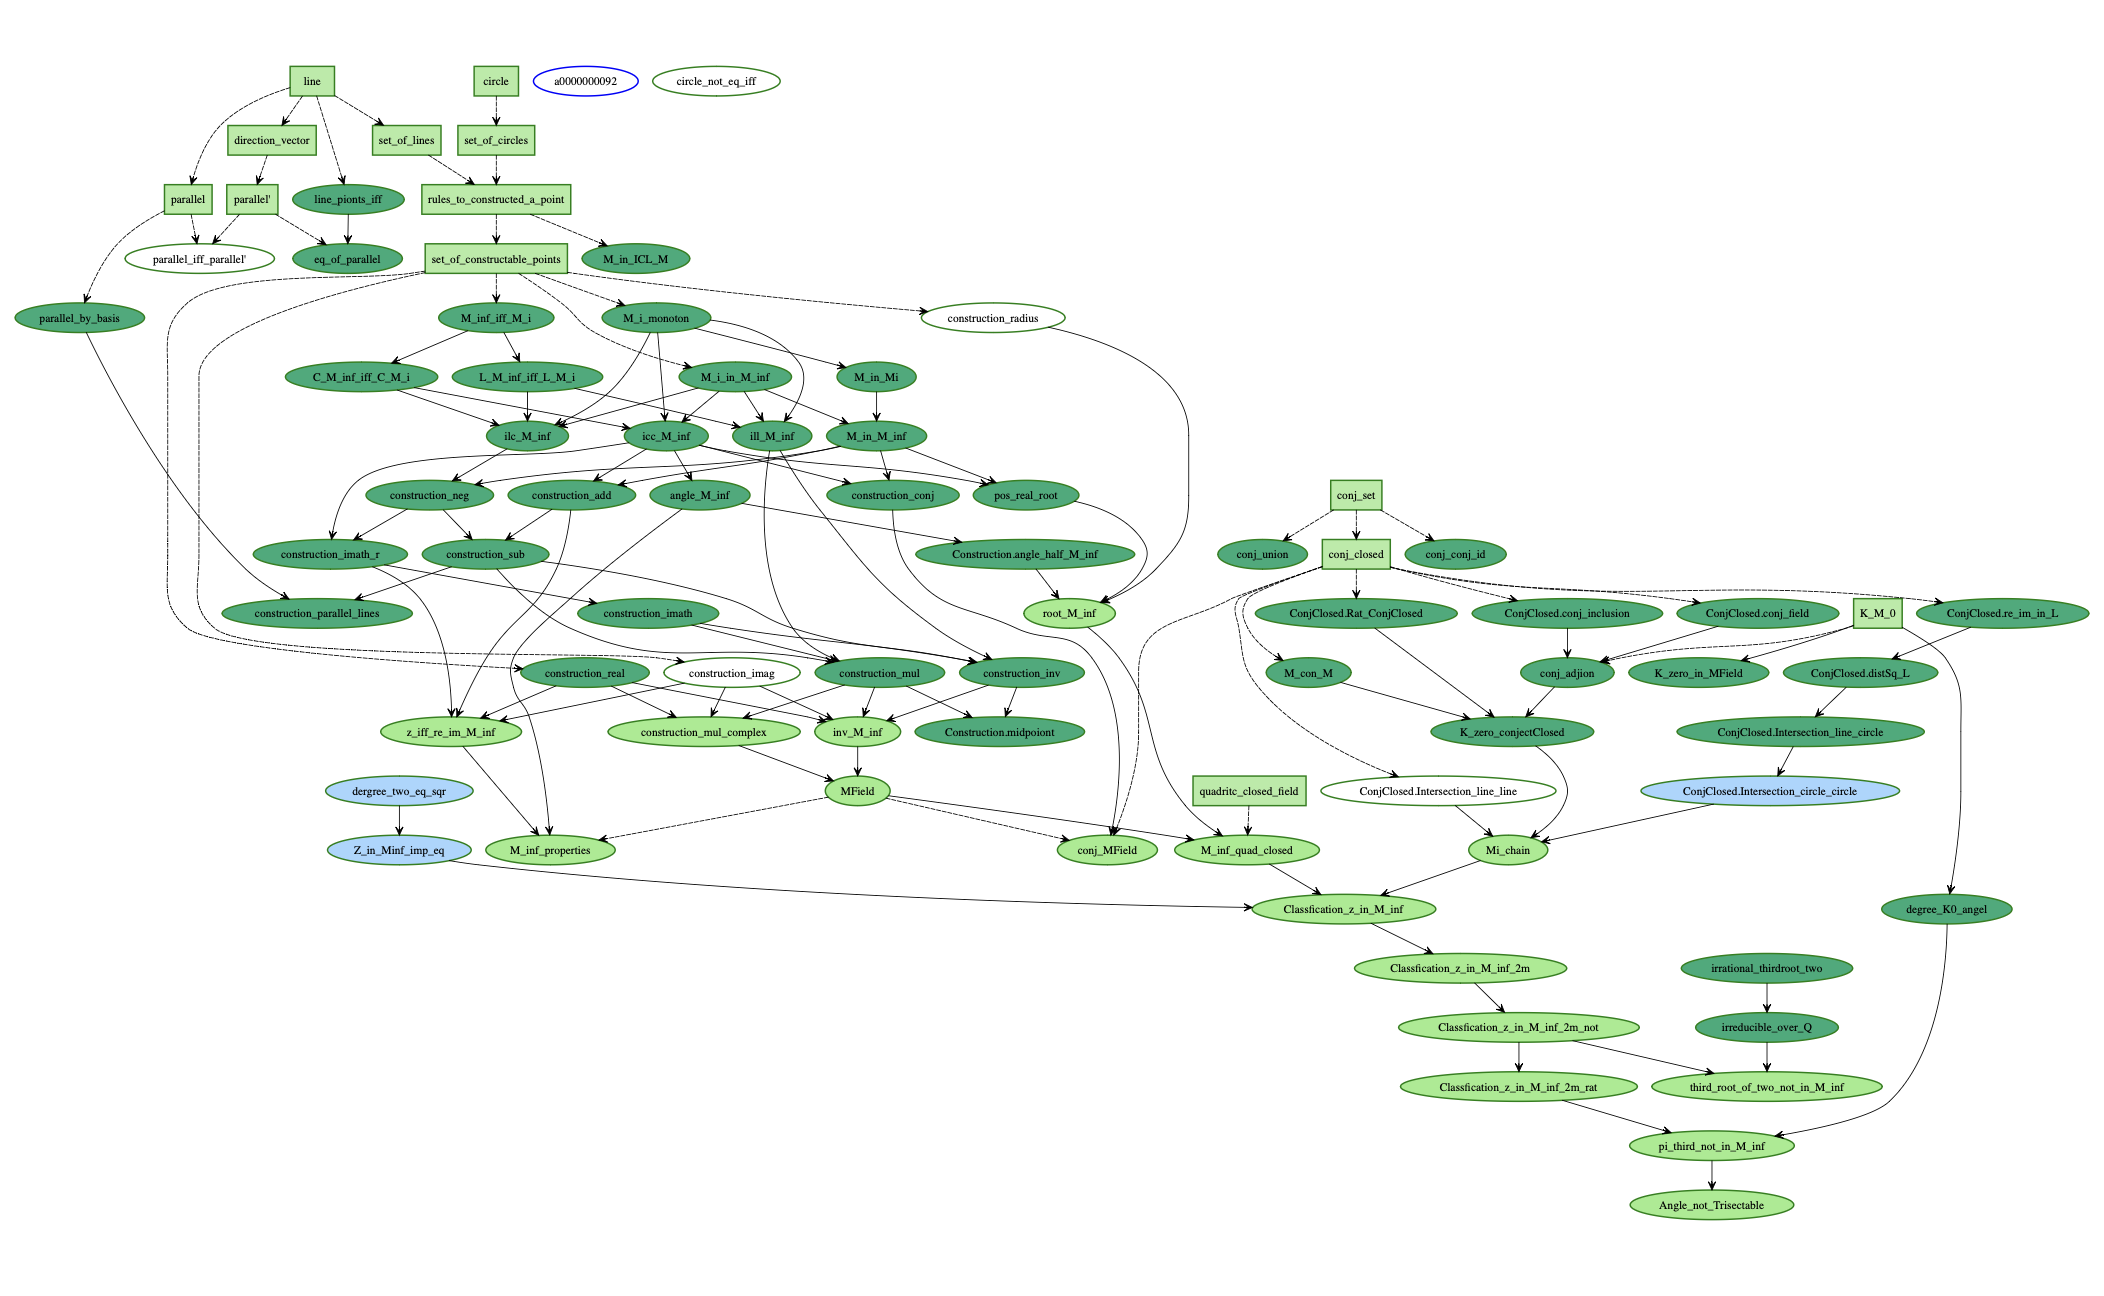
\includegraphics[angle=0]{slides/DependencyGraph}}
        \label{fig:DependencyGraph}
        \caption{Dependency Graph}
    \end{figure}
\end{frame}
\section{Classification}
\begin{frame}
    \begin{definition}
        \label{def:K_M_0}
        \lean{K_zero}
        \leanok
        Let $\mathcal(M)\subseteq\mathbb{C}$ with $0,1 \in \mathcal{M}$. Define:
        \begin{equation*}
            K_0 := \mathbb{Q}(\mathcal{M}\cup Conj(\mathcal{M}))
        \end{equation*}
    \end{definition}
\end{frame}

\begin{frame}
    \begin{theorem}[constructable iff chain dergee2]
        \label{thm:Classfication_z_in_M_inf}
        \lean{Classfication_z_in_M_inf, adjoin_in_MField'}
        \leanok
        For $z \in \mathbb{C}$, $z \in M_{\infty}$ is equivalent to:\\
        There is a $0\le n$ and a chain 
        $$K_0 = L_1 \subset L_2 \subset \ldots \subset L_n \subset \mathbb{C}$$
        of subfields of $\mathbb{C}$ such that $z \in L_n$ and 
        $$ [L_{i+1}:L_i] = 2 \quad \text{for} \quad i = 0, \ldots, n-1.$$
    \end{theorem}

    
\end{frame}

\begin{frame}
    \begin{corollary}
        If $z \in M_{\infty}$, then there exists an $m\in \N$ such that $[z:\mathcal{K}_0] = 2^m$.
    \end{corollary}

\begin{corollary}[Classfication]
    If there is no $m\in \N$ such that $[z:\mathcal{K}_0] = 2^m$, then $z \notin M_{\infty}$.
\end{corollary}

\end{frame}
\section{Impossibility of doubling the cube}
\section{Doubling the cube}
The doubling of the cube, also known as the Delian problem, represents an ancient geometric problem.
The objective is to construct the edge of a second cube whose volume is double that of the first, using only a ruler and compass, given the edge of a cube.
The construction of a second cube with double the volume of the original cube begins with a cube of volume $a^3$, where $a$ is the length of an edge. 
Thus, a cube with double the volume ($2\cdot a^3$) has an edge length of the cube root of two times the length of the original edge.
If we now take the unit cube and reduce $\mathcal{M}$, the problem is as follows:
\begin{problem}
    Let $\mathcal{M} = \{0,1\}$.  
    $$\text{Is }\sqrt[3]{2} \overset{?}{\in} \mathcal{M}_{\infty}?$$
\end{problem}

\begin{lemma}($\sqrt[3]{2}$ is irrational)
    \label{lem:irrational_thirdroot_two}
    \leanok
    \lean{irrational_thirdroot_two}
    The third root of $2$ is an irrational number.
\end{lemma}
\begin{proof}
    \leanok
    The following theorem will be used without proof, as it is already available in MathLib:
    \begin{theorem*}
        For any $x\in(\R\setminus\Z)$ if there exist an $n\in \N_{>0}$ and $m\in\Z$ such that $m = x^n$, then $x$ is rational. 
    \end{theorem*}
    The fact that $(\sqrt[3]{2})^3=2$, allows us to deduce that the only remaining task is to prove that it  is not an integer. 
    This can be observed trough two relations.
    \begin{align}
        2^{\frac{1}{3}} &< 2 \\
        2^{\frac{1}{3}} &> 1
    \end{align}
\end{proof}

\begin{lemma}
    $P := X^3 - 2$ is irreducible over $\mathbb{Q}$.
\label{lem:irreducible_over_Q}
\leanok
\lean{P_irreducible}
\end{lemma}
\begin{proof}
    \leanok
    \uses{lem:irrational_thirdroot_two}
    Since $\mathbb{Q}$ is $a$ subfield of $\mathbb{C} [X]$, we know that
    \begin{equation*}
        X^3 - 2 = (X - \sqrt[3]{2})(X -\zeta_3 \sqrt[3]{2})(X -\zeta_3^2 \sqrt[3]{2})
    \end{equation*}
    Suppose $P$ is reducible, then
    \begin{equation*}
        X^3 - 2 = (X - a)(X^2 + bX + c)\text{, with } a, b, c \in \mathbb{Q}
    \end{equation*}
    In particular it has a zero in $\mathbb{Q}$, so there is a rational number $a$ such that $a^3 = 2$.\newline
    But we know that $\zeta_3 \sqrt[3]{2}$ and $\zeta_3^2 \sqrt[3]{2}$ are not real numbers and $\sqrt[3]{2}$ is not rational \ref{lem:irrational_thirdroot_two}.
    So $P$ is irreducible over $\mathbb{Q}$.
\end{proof}

\begin{theorem}
    \label{thm:third_root_of_two_not_in_M_inf}
    \leanok
    \lean{third_root_of_two_not_in_M_inf}
    The cube can't be doubled using a compass and straightedge.
\end{theorem}
\begin{proof}
    \leanok
    \uses{lem:irrational_thirdroot_two, lem:irreducible_over_Q, cor:Classfication_z_in_M_inf_2m_not}
    By applying the corollary \ref{cor:Classfication_z_in_M_inf_2m_not}, it is sufficient to proof that no $m\in \N$ exists such that
    $$2^m\overset{?}{=}[\sqrt[3]{2}:\Q({0,1})]\overset{0,1\in\Q}{=} [\sqrt[3]{2}:\Q] = \text{degree}(\mu_{\Q,\sqrt[3]{2}}).$$
    Since $P$ is irreducible over $\mathbb{Q}$ \ref{thm:irreducible_over_Q}, monic and has $\sqrt[3]{2}$ as a zero, we know that $[\mathbb{Q}(\sqrt[3]{2}):\mathbb{Q}] = 3$.
    And since $$ 3  \equiv_2 1 \neq 0  \equiv_2 = 2^m \qquad\forall m \in \N$$
    we can conclude that the cube can't be doubled using a compass and straightedge.
    
\end{proof}

\section{Trisection of an angle}
The trisection of an angle with a compass and ruler can be reduced to the following problem:\\
Let $\mathcal{M} = \{a, b, c\}$ with $a, b, c$ not on a line and $\alpha := \angle (b - a, c - a)$ be the resulting angle.
Then $\alpha$ can be trisected if and only if there is a point $d\in \mathcal{M}_{\infty}$ such that $\angle (b - a, d - a) = \alpha/3$. 
The use of a normed set $\mathcal{M} = \{0,1,e^{i\alpha}\}$ leads to the following problem:
\begin{problem}
    Let $\mathcal{M} = \{0,1,\exp(\textbf{i} \alpha)\}$. $$\text{Is }\exp(\textbf{i} \alpha/3) \overset{?}{\in} \mathcal{M}_{\infty}?$$
\end{problem}
In this context, since the numbers zero and one are rational numbers, it can be concluded that $K_0$ is equal to
$$ K_0 = \mathbb{Q}(\mathcal{M}\cup Conj(\mathcal{M})) = \mathbb{Q}(e^{\imath\alpha},\overline{e^{\imath\alpha}}). $$
Given the corollary reference and the fact that $e^{\imath\alpha/3}$ is a zero of $X^3 - e^{\imath\alpha}\in \mathbb{Q}(e^{\imath\alpha},\overline{e^{\imath\alpha}})[X]$, the following is  equivalent: 
\begin{itemize}
    \item $\exp(\textbf{i} \alpha/3) \notin \mathcal{M}_{\infty}$
    \item $\text{degree}(\mu_{e^{\imath\alpha/3},K_0}) = 3$
    \item $X^3 - e^{\imath\alpha}$ is irreducible over $\mathbb{Q}(e^{\imath\alpha},\overline{e^{\imath\alpha}})$
\end{itemize}
The following section will demonstrate that the angle of $\frac{\pi}{3}=60°$  is not trisectable.

\begin{lemma}
    \label{lem:degree_K0_angel}
    \leanok
    \lean{degrre_root_three, eaual_adjion_root_three}
    The degree of $K_0 = \mathbb{Q}(e^{\imath\frac{\pi}{3}},\overline{e^{\imath\frac{\pi}{3}}})$ is equal  to $2$. 
\end{lemma}
\begin{proof}
    \leanok
    \uses{def:K_M_0}
    For all real numbers $\alpha$, we have that  $$ \exp(\imath \alpha) = \cos(\alpha) + \imath \sin(\alpha).$$
    For $\alpha = \pi / 3$ we get
    \begin{equation*}
        \cos(\alpha) = \frac{1}{2}\qquad \text{and}\qquad \sin(\alpha) = \frac{\sqrt{3}}{2}
    \end{equation*}
    Therefore $\mathbb{Q}(e^{\imath\frac{\pi}{3}},\overline{e^{\imath\frac{\pi}{3}}})$ is in $\mathbb{Q}(\imath\sqrt{3})$.
    And since $\imath\sqrt{3}$ is a zero of $X^2 + 3$, we know that the degree of $K_0$ less then $2$.
    To show that the degree is not $1$, we apply the fact that $\imath\sqrt{3} \notin \mathbb{Q}$.
    % Since we know that $\sqrt{r} \in \mathcal{M}_{\infty}$ for $r \in \mathcal{M}_n$
    % we see that $\exp(\textbf{i} \alpha) \in \mathcal{M}_{\infty}$ for $\mathcal{M} = \{0,1\}$. \newline
    % So we will work with $K_0 = \mathbb{Q}$.
\end{proof}

\begin{lemma}
    \label{lem:pi_third_not_in_M_inf}
    \leanok
    \lean{pi_third_not_in_M_inf}
    The angle $\pi / 3 = 60^{\circ}$ can't be trisected using a compass and straightedge.
\end{lemma}
\begin{proof}
    \leanok 
    \uses{lem:degree_K0_angel, cor:Classfication_z_in_M_inf_2m_rat}
    By utilising the aforementioned lemma \ref{lem:degree_K0_angel} to apply the corresponding corollary \ref{cor:Classfication_z_in_M_inf_2m_rat}, we can narrow our focus to the degree over $\Q$.
    Now we use the fact that if $x\in \mathcal{M}_{\infty}$, then $x.real, x.imag \in \mathcal{M}_{\infty}$ \ref{lem:M_inf_properties}. 
    Thus we focus on $\cos(\alpha/3)$, which the real part $e^{\imath \frac{\pi}{3}}$ and a zero of
    \begin{equation*}
        f := 8 X^3 - 6 X - 1 \in \mathbb{Q}[X]
    \end{equation*}
    Suppose $f$ is reducible over $\mathbb{Q}$, then $f$ has a rational zero $a$, since $f$ is of degree $3$. According to the rational root theorem, a root rational root of $f$ is of the form $\pm \frac{p}{q}$ with $p$ a factor of the constant term and $q$ a factor of the leading coefficient. So the only possible rational zeros of $f$ are
     \begin{equation*}
        \{ \pm 1, \pm \frac{1}{2}, \pm \frac{1}{4}, \pm \frac{1}{8} \}.
     \end{equation*}
     One can check that none of these numbers are a zero of $f$.
     So $f$ is irreducible over $\mathbb{Q}$ and $\cos(\alpha/3) \notin \mathcal{M}_{\infty}$.
     Therefore
        \begin{equation*}
            \exp(\textbf{i} \alpha/3) \notin \mathcal{M}_{\infty}
        \end{equation*}
    So the angle $\pi / 3 = 60^{\circ}$ can't be trisected using a compass and straightedge.
\end{proof}

\begin{theorem}
    \label{thm:Angle_not_Trisectable}
    \leanok
    \lean{Angle_not_Trisectable}
    A general angle can't be trisected using a compass and straightedge.
\end{theorem}
\begin{proof}
    \leanok
    \uses{lem:pi_third_not_in_M_inf, }
    Employ the previous lemma with the angle $\pi / 3$.
\end{proof}
\begin{frame}[allowframebreaks]{References}
    \bibliography{construct}
    \bibliographystyle{plainurl}
  \end{frame}
\nocite{*}
\end{document}